% This work by Jeremy A. Hansen is licensed under a Creative Commons 
% Attribution-NonCommercial-ShareAlike 3.0 Unported License, 
% as described at http://creativecommons.org/licenses/by-nc-sa/3.0/legalcode

\LevelD{Introduction}

Okay, so you know how to do some programming, but now you need to be able to handle a dozen or more operations that are obnoxiously repetitive.
Imagine that you have a program that needs to allow data to be entered about your employees.
Do you really want to have to write out the code to do that for every single individual?
No---you want to set it up so you write it out as concisely as possible, and copy and paste just won't work.
What we need to do is write the relevant code once and have it repeated for us as many times as necessary.

For this, we'll use a structure known as a \Keyword{loop}, which does exactly what you expect it would.
A loop allows you to repeat a section of code as many times as you need.
When the code reaches the end of the section, it goes back to the top of the section and the loop starts again.
After each repetition of the loop (which we call an \Keyword{iteration}), it will check for an \Keyword{end condition} that is specified by the programmer. 

\LevelD{Having Fun \Code{while} Programming}

The first loop we'll cover is the \Code{while} loop, probably the simplest and easiest-to-use loop.
It's referred to as a \Keyword{pretest loop} as it's designed to check the loop's end condition prior to a repetition of the loop.

\begin{figure}[tbh]
  \centering
  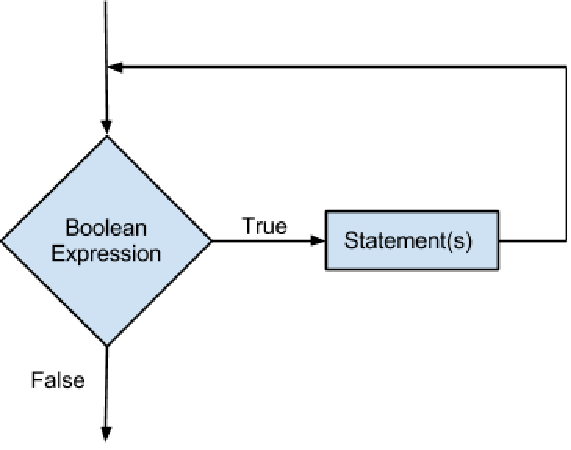
\includegraphics[width=0.7\textwidth]{diagrams/while_logic.pdf}
  \caption{Logic of a \Code{while} loop} \label{fig-while-logic} 
\end{figure}

In Figure \ref{fig-while-logic}, the basic model of a \Keyword{pretest loop} is shown.
A diamond is used to represent where a decision must be made.
In this case, it's a Boolean expression.
If the expression is true, control passes to the rectangle, which represents an action (or actions) to be performed: the statements that represent the body of the loop.

As with everything else we've learned so far, syntax is important. The structure is simple enough, as the pseudocode below shows:

\noindent\begin{minipage}{\linewidth}\begin{lstlisting}
while (BooleanExpression)
{
  statement;
  statement;
  // whatever else needs to be done
}
\end{lstlisting}\end{minipage}

The important thing to remember here is to be sure you have some statement to eventually allow the loop to exit.
When the Boolean expression is false, remember, the loop is finished.

Also, note that, like an \Code{if} statement, the braces are not necessary if there is only one statement following the line with the \Code{while} keyword and Boolean expression.
Is it recommended to use the braces with only one statement?
For your own sanity, and that of others reading your code, yes.
Do you have to?
No, but some organization's coding standards might say otherwise, because it makes the code easier to read and edit.
So remember, it's best to start with good habits early.

Now, let's look at an actual example of a \Code{while} loop. \nopagebreak[4]

\noindent\begin{minipage}{\linewidth}\begin{lstlisting}
int i = 10;	//initializes i at 10

cout << "T-minus ";
// while loop that is ended when i is less than 0
while(i>=0)	
{ 
  //outputs the value of i, then moves to a new line
  cout << i << endl;	
  //decreases the value of i by 1
  i--;	
};

cout << "Lift Off!";
\end{lstlisting}\end{minipage}

This code prints a countdown:

\noindent\Code{10}

\noindent\Code{9}

\noindent\Code{8}

\noindent\Code{7}

\noindent\Code{6}

\noindent\Code{5}

\noindent\Code{4}

\noindent\Code{3}

\noindent\Code{2}

\noindent\Code{1}

\noindent\Code{Lift Off!}

\LevelD{\Code{do}-\Code{while} Loops}

Remember how the \Code{while} loop is known as a pretest loop?
Well, a \Code{do}-\Code{while} loop is known as a \Keyword{post-test loop} for a similar reason.
Let's take a look at the flowchart in Figure \ref{fig-do-while-logic} and take a guess.

\begin{figure}[tbh]
  \centering
  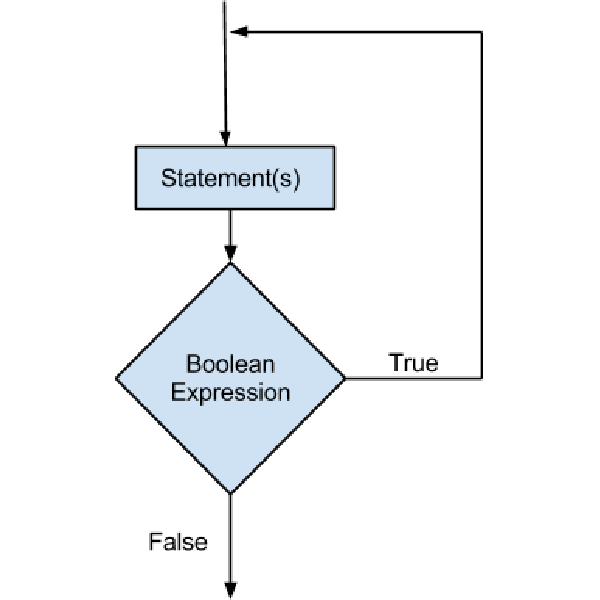
\includegraphics[width=0.7\textwidth]{diagrams/do_while_logic.pdf}
  \caption{Logic of a \Code{do}-\Code{while} loop} \label{fig-do-while-logic} 
\end{figure}

Post-test loops perform the statements in the body of the loop \emph{before} it tests the end condition.
Let's look how this will affect the syntax you will use when implementing the loop.

\noindent\begin{minipage}{\linewidth}\begin{lstlisting}
do
{
  something;
  something;
  // whatever else needs to be done
} while (BooleanExpression)
\end{lstlisting}\end{minipage}

The difference between a \Code{while} and a \Code{do}-\Code{while} loop is where each checks its end condition.
In this case, the line with the \Code{while} and the end condition are after the main section of code.
In a normal \Code{while} loop, the program can potentially meet the end condition before even entering the loop body, and just pass over it.
In a \Code{do}-\Code{while} loop, the program checks the end condition after each iteration of the loop, so it will run at least once before the loop ends.

There's not a whole lot more to add then hasn't been stated in the while loop section, so here's an example.

\noindent\begin{minipage}{\linewidth}\begin{lstlisting}
char cont; // Short for continue; 
           // continue is a key word and can't be used

do {
  cout << "Go Cadets!\n";
  cout << "Do you want to continue? Type Y for yes: \t";
  cin >> cont;
} while (cont == 'Y');
\end{lstlisting}\end{minipage}

\LevelD{Event-Based Loops vs Count-Based Loops}

Loops can be organized into two categories based on how you use them.
These two categories are defined by if you want to do a certain number of iterations of the loop (a \Keyword{count-controlled} loop) or continue until some event occurs, such as a particular user input (an \Keyword{event-controlled} loop).
Let's look at code examples to differentiate the two. The first example shows an event-controlled \Code{while} loop.

\noindent\begin{minipage}{\linewidth}\begin{lstlisting}
// Declares sum and temp. Initializes sum to 0.
int sum=0, temp; 

cout << "Please give a number to add: ";
// User inputs into a temporary variable to add to sum
cin >> temp;	

while (temp != 0) 
{
  // Sets sum equal to sum+temp at start of loop
	sum += temp;	
	cout << endl << "total: " << sum << endl;	
  //asks user to input temp variable again
	cout << "Add another number? If yes, input "
    << "a nonzero integer. If no, input 0." << endl;	
  cin >> temp;
}
\end{lstlisting}\end{minipage}

\noindent This example shows a count-controlled \Code{while} loop:

\noindent\begin{minipage}{\linewidth}\begin{lstlisting}
int counter = 1;

while(counter != 12)
{
  cout << counter << endl;
  counter++;
}
\end{lstlisting}\end{minipage}

\LevelD{\Code{for} work or \Code{for} play}

Consider what we have needed for each loop we've covered.
We've needed to initialize a variable that we want to check.
We've also needed an end condition to test that variable against.
Finally, we needed a way of modifying that variable to meet that end condition.
After that, it's whatever we've felt like putting in. With the \Code{for} loop, we put those three elements into the loop header, separated by semicolons (\Code{;}).
A \Code{for} loop would would look something like this:

\noindent\begin{minipage}{\linewidth}\begin{lstlisting}
for(Intialization; Test; Update)
{
  something;
  something;
  // whatever else you need
}
\end{lstlisting}\end{minipage}

The \Code{for} loop by its nature lends itself to being a count-controlled loop.
You use this kind of loop to count up (or down) each iteration until you get to the specified value. 

Let's run through how a \Code{for} loop should run, following the code below.
Assuming everything is correct, you would initialize the first value to something such as an \Code{int counter} that is set to 1.
The \Code{TestExpression} will include the same Boolean logic you would use in \Code{while} and \Code{do}-\Code{while} loops, so let's just say when \Code{counter} is less than or equal to 5, the loop will terminate.
Finally, let's say  \Code{counter++} is the update expression.
In each iteration (unless you also decide to change \Code{counter} from the body of the loop) you will move through this pretest loop four times.

\begin{figure}[tbh]
  \centering
  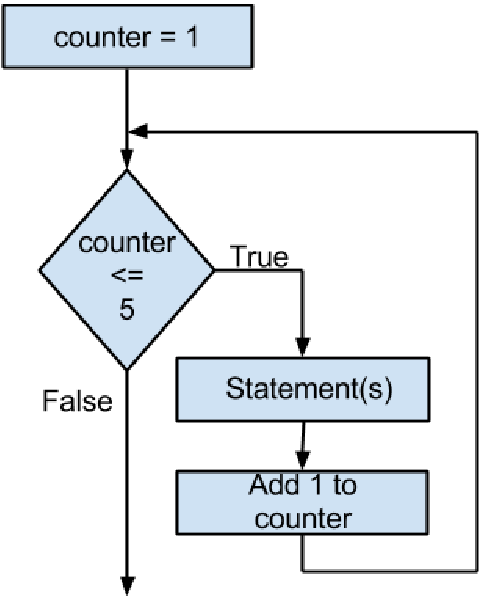
\includegraphics[width=0.7\textwidth]{diagrams/for_logic.pdf}
  \caption{Logic of a \Code{for} loop} \label{fig-for-logic} 
\end{figure}

\noindent This code corresponds to the logic in Figure \ref{fig-for-logic}:

\noindent\begin{minipage}{\linewidth}\begin{lstlisting}
for(int counter = 1; counter <= 5; i++)
{
  cout << i << endl;
}
\end{lstlisting}\end{minipage}

\noindent ...which produces the following output:

\noindent\Code{1}

\noindent\Code{2}

\noindent\Code{3}

\noindent\Code{4}

\noindent\Code{5}

\LevelD{Picking a Loop}

Which loop you use is dependent on your preferences and needs.
A \Code{for} loop is nice, but it's more convenient as a count-controlled loop.
If you needed to use an event-controlled loop, you may prefer to use a \Code{while} or \Code{do}-\Code{while} loop.
A \Code{for} loop is a nice way to condense the initialization, end conditions and update statement of the loop into one short line.
When choosing between a \Code{do}-\Code{while} and a \Code{while} loop, you should remember that with a \Code{do}-\Code{while}, it will always run at least once, while a \Code{while} loop may run zero or more times.

\LevelD{Nested Loops}

Much like \Code{if} statements, loops can be nested within each other.
Just remember to practice good formatting habits to keep the code from being too confusing.
Take a look at the example below, then let's talk our way through it. \nopagebreak[4]
 
\noindent\begin{minipage}{\linewidth}\begin{lstlisting}
//a single day
for(int hours = 0; hours < 24; hours++)	
{
  // a single hour
  for(int minutes = 0; i < 60; minutes++)	
  {
    //a single minute 
    for(int seconds = 0; seconds < 60; seconds++) 	
    {
      //outputs the current time
      cout << hours << ":" << minutes
        << ":" << seconds << endl;
		}
	}
}
\end{lstlisting}\end{minipage}

For those readers who concluded that this is a clock simulation, you are correct!
Our system of time is set up that we have 24 hours in a day, and each hour needs to go through a 60 minute cycle, and each minute has a 60 second cycle.
The code mimics this by advancing the seconds 60 times before advancing each minute.
After 60 minutes, the hour counter loop is incremented. Each time an outer loop starts another iteration, variables inside the inner loops are reset.

\LevelD{Infinite Loops}

Remember to have some way of advancing towards the end condition.
What will happen if you can't reach that end condition from within the loop?
Most likely an infinite loop will occur. And what exactly is an infinite loop?
If you said it's a loop that can't stop itself, then you would be right.
Depending on the operation of the loop, you may not know what is happening, and this could potentially cause disastrous results.
Let's look at an example of a \Code{while} loop that suffers from an infinite loop.

\noindent\begin{minipage}{\linewidth}\begin{lstlisting}
int counter = 1;

while(counter != 12)
{
  cout << counter << endl;
  counter += 2;
}
\end{lstlisting}\end{minipage}

Because \Code{counter} starts with a value of 1, and adds 2 each time the loop executes, \Code{counter} will always be odd, and never equal twelve.
Therefore, the loop will never end.

\LevelD{Review Questions}
\begin{enumerate}
\item Create a \Code{while} loop that increments some integer variable \Code{x} initialized with a value of 0 by 3 until the value of \Code{x} reaches a value of 30.
Make sure you declare the variable and initialize it first! 

\item  Create a \Code{do}-\Code{while} loop that reads integer values given by the user into an integer variable \Code{x}, initialized to 0, then adds those values onto some variable named \Code{totalVal} until \Code{totalVal} reaches at least 20.

\item Create a \Code{for} loop that outputs your name to the screen 10 times before exiting the loop.

\item Spot the logic error and correct it in the following code:

\noindent\begin{minipage}{\linewidth}\begin{lstlisting}
for(int j = 10, j > 0, j--)
{
  cout << j << endl;
  if (j = 1)
  {
    cout << "BOOM!\n";
  }
}
\end{lstlisting}\end{minipage}

\item In the last question, was the loop an event-controlled loop or count-controlled loop?
\end{enumerate}


\LevelD{Review Answers}
\begin{enumerate}

\item
\noindent\begin{minipage}{\linewidth}\begin{lstlisting}
int x = 0;
while (x < 10)
{
  x++;
} 
\end{lstlisting}\end{minipage}

\item
\noindent\begin{minipage}{\linewidth}\begin{lstlisting}
int x = 0;
int totalVal = 0;
do
{
  cout << "Type in a number: "; 
  cin >> x;
  totalVal += x;
}
while (totalVal < 20); 
\end{lstlisting}\end{minipage}

\item 
\noindent\begin{minipage}{\linewidth}\begin{lstlisting}
for(int i = 0; i < 10; i++)
{
  cout << "Your name here\n";
}
\end{lstlisting}\end{minipage}

\item
\noindent\begin{minipage}{\linewidth}\begin{lstlisting}
for (int j = 10; j > 0; j--)
{
  cout << j << endl;
  if (j == 1)
  {
    cout << "BOOM!\n";
  }
}
\end{lstlisting}\end{minipage}

\item Count-controlled

\end{enumerate}


\LevelD{Further Reading}
Basic Loops:
\begin{itemize}
\item \url{http://www.cplusplus.com/doc/tutorial/control/}
\item \url{http://www.cprogramming.com/tutorial/lesson3.html}
\end{itemize}

\noindent Ranged-Based Loops
\begin{itemize}
\item \url{http://www.cprogramming.com/c++11/c++11-ranged-for-loop.html}
\end{itemize}


